%%%%%%%%%%%%%%%%%%%%%%%%%%%%%%%%%%%%%%
%%%%%%%%%%%%%%%%%%%%%%%%%%%%%%%%%%%%%%
% Do not edit the TeX file your work
% will be overwritten.  Edit the RnW
% file instead.
%%%%%%%%%%%%%%%%%%%%%%%%%%%%%%%%%%%%%%
%%%%%%%%%%%%%%%%%%%%%%%%%%%%%%%%%%%%%%




% TODO: define these in knitr instead.
\global\long\def\splinedegree{3}
\global\long\def\ntime{14}
\global\long\def\ngenes{1000}
\global\long\def\nclusters{18}
\global\long\def\fullparamdim{66199}
\global\long\def\covregularization{0.1}

\global\long\def\regmat{X_{df}}
\global\long\def\mbe{\mathbb{E}}
\global\long\def\cov{\mathrm{Cov}}
\global\long\def\thetareg{\theta_{r}}
\global\long\def\thetaclust{\theta_{c}}

We start with some DP prior parameter $\alpha_0$. After choosing a different
$\alpha$, we compare the posterior expected number of clusters (
\prettyref{eq:expected_num_clusters}) predicted by our linear approximation
against the expectation obtained from re-optimizing the objective. The results
are shown in \prettyref{fig:parametric_sens_e_num_clusters}.

More specifically, we evaluated the expected number of clusters for a range of
$\alpha$ between 0.5 and 6.5. Then we chose three $\alpha_0$ values, 2, 3.5, and
5, and constructed the linear approximation centered at each of these
$\alpha_0$s. The linear approximation did quite well for choices of $\alpha$
close to $\alpha_0$. Hence, by evaluating the objective at three $\alpha_0$s, we
can use the linear approximation to understand the effect of the DP prior
parameter $\alpha$ across the entire range from 0.5 - 6.5.


\begin{knitrout}
\definecolor{shadecolor}{rgb}{0.969, 0.969, 0.969}\color{fgcolor}\begin{figure}[!h]

{\centering 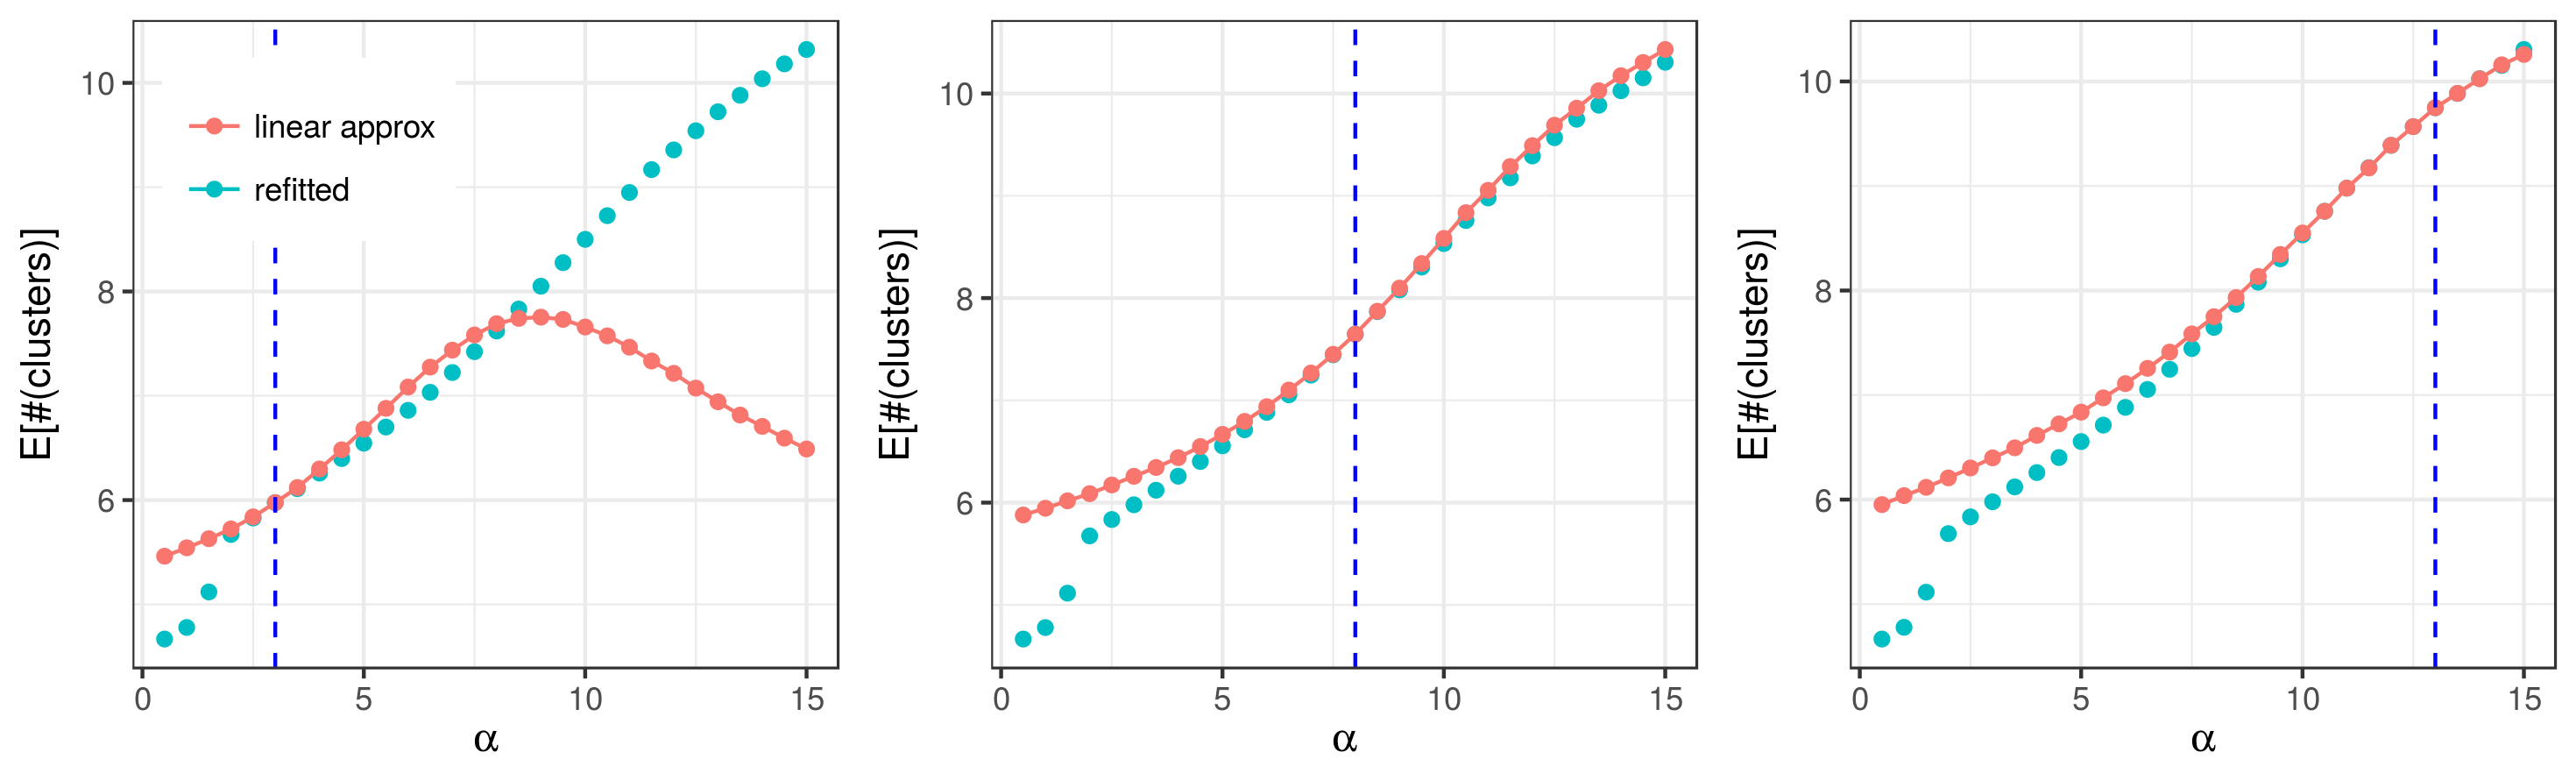
\includegraphics[width=0.98\linewidth,height=0.343\linewidth]{figure/parametric_sens_plot-1} 

}

\caption{\label{fig:parametric_sens_e_num_clusters}Comparison of the expected number of clusters computed by re-optimizing
  the variational objective for various epsilon perturbations to the BNP prior parameter
  (green),
  versus the predicted value from our linear approximation (orange), with alpha0 the
  blue horizontal line.}\label{fig:parametric_sens_plot}
\end{figure}


\end{knitrout}


\subsection{Functional perturbations}
%
We now use the functional perturbation described in
\prettyref{eq:expon_perturb} to perturb the prior on the stick distribution. The
results are shown in \prettyref{fig:func_sens_e_num_clusters}.

We chose two different functional perturbations: for the first we let
$p_1(\nu_k)$ be a logit normal with parameters $\mu = -2, \sigma = 1$; for the
second, we let $p_1(\nu_k)$ be a logit normal with parameters $\mu = 2, \sigma =
1$. In both cases, we then chose $\phi(\nu_k) = p_1(\nu_k) / p_{0k}(\nu_k)$.



\begin{knitrout}
\definecolor{shadecolor}{rgb}{0.969, 0.969, 0.969}\color{fgcolor}\begin{figure}[!h]

{\centering 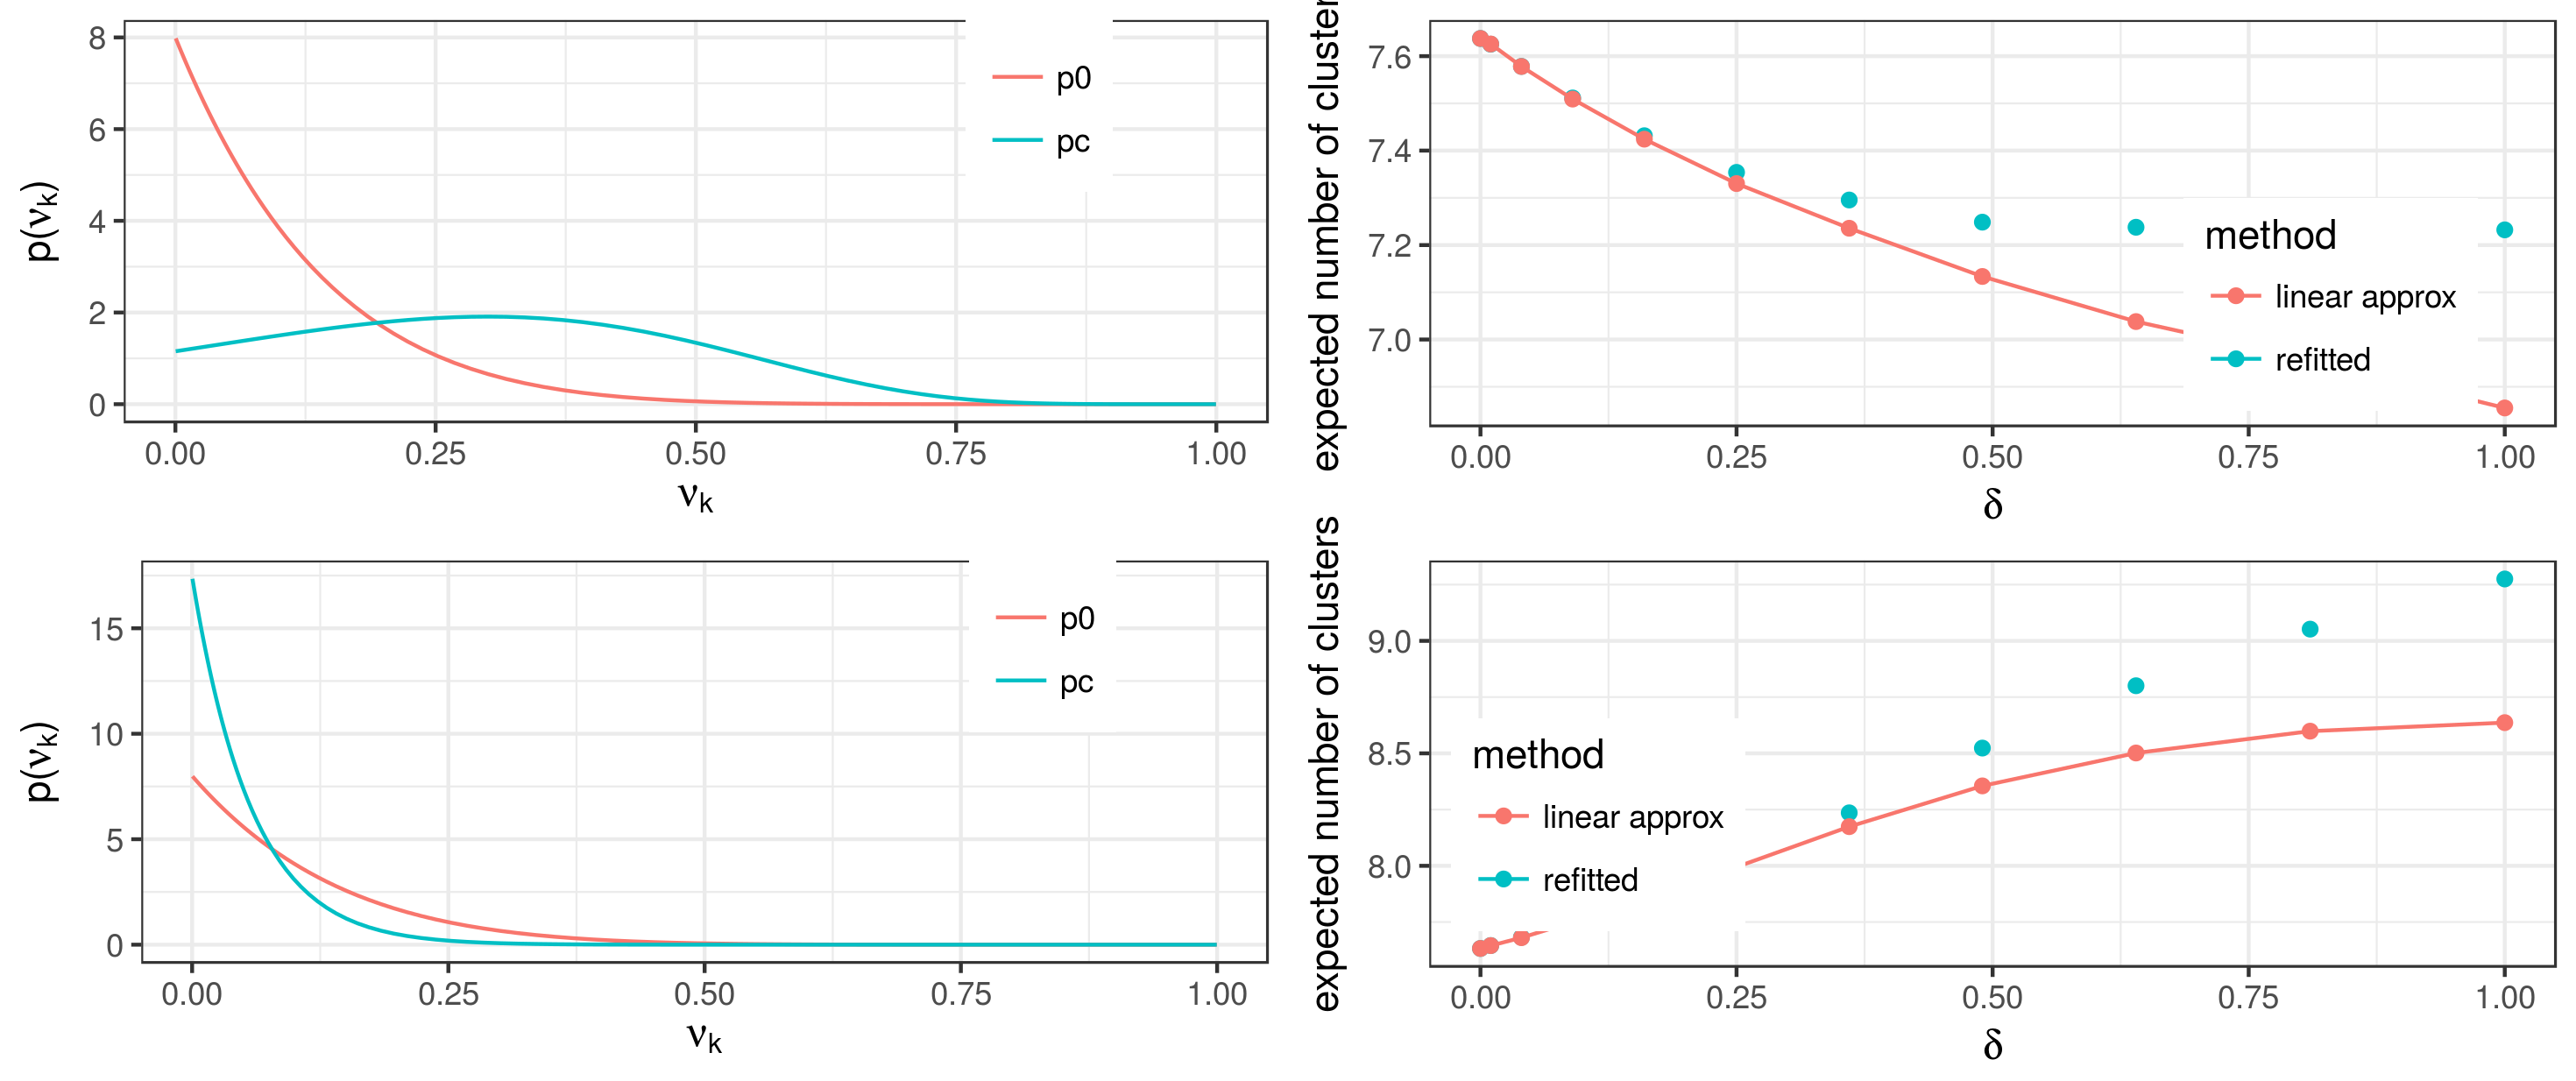
\includegraphics[width=0.98\linewidth,height=0.686\linewidth]{figure/functional_sens_plot-1} 

}

\caption{\label{fig:func_sens_e_num_clusters}
Left column: the original prior p0 in purple, the perturbed prior pc in red. Right: linearly approximated vs.
re-fitted expected number of clusters after the purtubation.  }\label{fig:functional_sens_plot}
\end{figure}


\end{knitrout}



% \begin{figure}[h!]
% 	\centering
% 	\begin{subfigure}[t]{0.32\textwidth}
% 		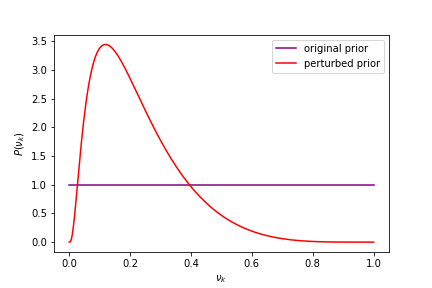
\includegraphics[width = \textwidth]{./functional_sens_results/perturbed_prior1_init3_5.png}
% 		\subcaption{}
% 	\end{subfigure}
%   \begin{subfigure}[t]{0.32\textwidth}
%     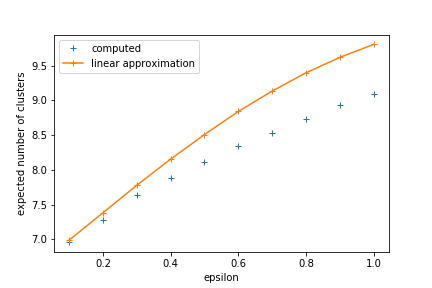
\includegraphics[width = \textwidth]{./functional_sens_results/pred_num_clusters1_init3_5.png}
%     \subcaption{}
%   \end{subfigure}\\
%   \centering
%   \begin{subfigure}[t]{0.32\textwidth}
%     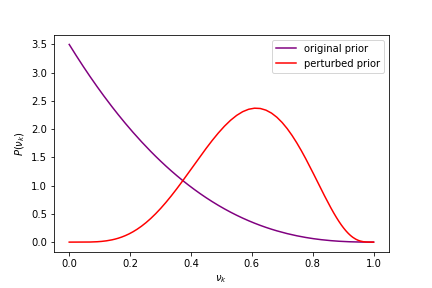
\includegraphics[width = \textwidth]{./functional_sens_results/perturbed_prior2_init3_5.png}
%     \subcaption{}
%   \end{subfigure}
%   \begin{subfigure}[t]{0.32\textwidth}
%     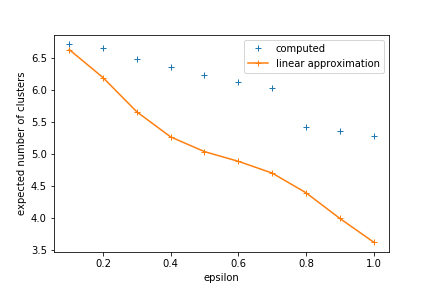
\includegraphics[width = \textwidth]{./functional_sens_results/pred_num_clusters2_init3_5.png}
%     \subcaption{}
%   \end{subfigure}
% 	\caption{Left column: the original prior in purple, the perturbed prior $p_1$ in red. Right: linearly approximated vs.
%   re-fitted expected number of clusters after purturbing each stick by $\phi(\nu_k)^\epsilon =
%   [p_1(\nu_k) / p_{0k}(\nu_k)]^\epsilon$.  }
% 	\label{fig:func_sens_e_num_clusters}
% \end{figure}
%
We find that the linear approximation in this case was able to capture the
direction of the perturbation, (expected number of clusters increased under the
first pertubation, decreased under the second), but did not provide a good
approximation at $\epsilon = 1$.
